\chapter{Results}
\label{chap:results}

\section{Dataset processing}
Eight miRNA-target chimera datasets have been previously generated for human, mouse, worm (\textit{Caenorhabditis elegans}), and cattle (\textit{Bos taurus}).
The details of each dataset are provided in Table \ref{tbl:dataset_description}, including the cell type or developmental stage that was examined and the experimental methods to obtain the data. Five of the datasets were generated by AGO-CLIP with an extra step to covalently ligate the miRNA and the target RNA (\textit{ca1}, \textit{ce1}, \textit{h1},  \textit{h3}, \textit{m2}). An additional \textit{C. elegans} dataset (\textit{ce2}) contains chimeras recovered from an iCLIP experiment that did not apply an additional ligation step. Two datasets (\textit{h2}, \textit{m1}) were generated by re-analysis of published mammalian AGO-CLIP data which also recovered miRNA-chimeras in libraries where no ligase was added \cite{grosswendt2014unambiguous}. The \textit{h2} and \textit{m1} datasets contain chimeras from a mix of 6 and 3 independent experiments, respectively.


\begin{table}[h!]
\caption{Datasets' information}
\label{tbl:dataset_description}
% \begin{tabular}{ | l | l | l | l | l | }
\begin{tabular}{|l|p{5cm}|p{4cm}|l|}
	\hline
	\textbf{Name} & \textbf{Cell/ Developmental stage} & \textbf{Experimental Method} & \textbf{Reference} \\
	\hline
	
% 	cattle\_MDBK & 
    ca1 &
	Madin-Darby bovine kidney (MDBK) &
	CLEAR-CLIP                        
	& \cite{scheel2017global} \\
	\hline
	
% 	celegans\_L3 & 
    ce1 &
	L3 staged & 
	Modified iPAR-CLIP & 
	\cite{grosswendt2014unambiguous}  \\
	\hline

% 	celegans\_L4 & 
    ce2 &
	Mid-L4 WT (N2)  & 
	ALG-1 iCLIP endogenous ligation & 
	\cite{broughton2016pairing} \\
	\hline

% 	human\_HEK293 & 
    h1 &
	Human embryonic kidney293 cells (HEK293) & 
	CLASH  & 
	\cite{helwak2013mapping} \\
	\hline
	
% 	human\_mix & 
    h2 &
	A mix of 6 datasets & 
	AGO-CLIP endogenous ligation &  
	\cite{grosswendt2014unambiguous} \\
	\hline
	
% 	human\_huh7.5 & 
    h3 &
	Human hepatoma cells (Huh-7.5) & 
	CLEAR-CLIP & 
	\cite{darnell_moore2015mirna} \\
	\hline
	
% 	mouse\_mix & 
    m1 &
	A mix of 3 datasets & 
	AGO-CLIP endogenous ligation & 
	\cite{grosswendt2014unambiguous} \\
	\hline
	
% 	mouse\_ATCC & 
    m2 &
	N2A mouse neuroblastoma (ATCC) & 
	CLEAR-CLIP & 
	\cite{darnell_moore2015mirna} \\
	\hline
\end{tabular}
\end{table}



We applied a multi-step processing pipeline (step 1) to retrieve all the required information about the interactions (e.g., miRNA name and sequence, target site sequence, and location). Since miRNA target sites that are located at the 3'UTRs of mRNA sequences are considered to be most functional \cite{menor2014mirmark, baek2008impact}, (step 2) we filtered out non 3'UTR interactions. Then (step 3) we generated miRNA-target duplexes using RNAduplex \cite{lorenz2011viennarna}. Finally (step 4) we classified the interactions based on their seed-pairing patterns and kept only interactions with canonical or non-canonical pairing patterns (see definitions in methods). 


The numbers of interactions that passed the pipeline stages are shown in Table \ref{tal:pipeline_summary}. The 3'UTR interactions represent 10\%-47\% of all interactions in the datasets and interactions with canonical or non-canonical seed-pairing constitute 53\%-82\% of them. The pipeline produced final datasets with variable sizes: four small datasets (500-1200), two large datasets (2000-5000), and two massive datasets ($\sim$18,000 each). These final datasets were later used as input for machine learning tasks. Therefore, we complemented the datasets with synthetically-generated negative interactions as described in methods. We extracted 490 features from each interaction, representing properties of the interaction duplex and interaction site and its flanking region within the 3'UTR (see methods: \nameref{methods_features}).


\begin{table}[h!]
\caption{Summary of the data processing pipeline}
      \label{tal:pipeline_summary}
                 \begin{threeparttable}
                    \resizebox{\textwidth}{!}{%

      \begin{tabular}{|l|l|l|l|l|l|l|l|l|}

\hline
\textbf{Dataset}                                                                                   & \textbf{ca1}     & \textbf{ce1}   & \textbf{ce2}   & \textbf{h1}     & \textbf{h2}     & \textbf{h3}     & \textbf{m1}    & \textbf{m2}      \\ \hline
No. of interactions \tnote{a}                                                                         & 296,297 & 3,627 & 4,920 & 18,514 & 10,567 & 32,712 & 1,986 & 130,094 \\ \hline
No. of interactions in 3'UTRs                                                                 & 30,534  & 1,704 & 1,206 & 8,507  & 2,039  & 4,634  & 902   & 33,100  \\ \hline
\textbf{\begin{tabular}[c]{@{}l@{}}Final dataset\\ (canonical \& non-canonical\\ interactions)\end{tabular}} & \textbf{18,204} & \textbf{1,176} & \textbf{992} & \textbf{5,137} & \textbf{1,150} & \textbf{2,846} & \textbf{537} & \textbf{17,574} \\ \hline
\end{tabular} }
\begin{tablenotes}
            \item[a] As provided by the original publications
        \end{tablenotes}
     \end{threeparttable}
\end{table}


\section{Datasets' characteristics}
In the following subsections we characterized the interactions of each dataset based on their miRNA distribution and base-pairing patterns. Since the negative interactions are synthetically-generated, we focused on positive interactions only.

\subsection{miRNA distribution}
We counted the appearance of miRNA sequences and miRNA seed families (nt2-7) and generated a distribution function for each dataset (Table \ref{tbl:mircontribution}). Our analysis indicates that the datasets are not uniformly distributed in terms of miRNA appearances (Figure \ref{fig:datasetplot}). Furthermore, 90\% of the interactions are dominated by a small subset of miRNA sequences (25-50\%) or miRNA seed families (18-37\%).



\begin{table}[h!]
\caption{Composition of miRNA sequences and miRNA seed families within datasets}
\label{tbl:mircontribution}
                    \resizebox{\textwidth}{!}{%

\begin{tabular}{|l|l|l|l|l|l|l|l|l|}
\hline
\textbf{Dataset}          & \textbf{ca1}                                                  & \textbf{ce1}                                                  & \textbf{ce2}                                                  & \textbf{h1}                                                   & \textbf{h2}                                                   & \textbf{h3}                                                   & \textbf{m1}                                                   & \textbf{m2}                                                    \\ \hline
\textbf{No. of interactions}   & 18,204  & 1,176 & 992   & 5,137  & 1,150  & 2,846  & 537   & 17,574                                                 \\ \hline
\textbf{No. of miRNA sequences}      & 165                                                  & 68                                                   & 56                                                   & 287                                                  & 140                                                  & 203                                                  & 98                                                   & 417                                                   \\ \hline
\textbf{90\% point [miRNA sequences]} & \begin{tabular}[c]{@{}l@{}}49 \\ (29\%)\end{tabular} & \begin{tabular}[c]{@{}l@{}}26 \\ (38\%)\end{tabular} & \begin{tabular}[c]{@{}l@{}}24 \\ (42\%)\end{tabular} & \begin{tabular}[c]{@{}l@{}}99 \\ (34\%)\end{tabular} & \begin{tabular}[c]{@{}l@{}}58 \\ (41\%)\end{tabular} & \begin{tabular}[c]{@{}l@{}}68 \\ (33\%)\end{tabular} & \begin{tabular}[c]{@{}l@{}}49 \\ (50\%)\end{tabular} & \begin{tabular}[c]{@{}l@{}}111 \\ (26\%)\end{tabular} \\  \hline
\textbf{No. of seed families}      & 119                                                  & 46                                                   & 35                                                   & 254                                                  & 133                                                  & 191                                                  & 88                                                   & 343                                                   \\ \hline
\textbf{90\% point [seed families]}  & \begin{tabular}[c]{@{}l@{}}21 \\ (18\%)\end{tabular} & \begin{tabular}[c]{@{}l@{}}14 \\ (30\%)\end{tabular} & \begin{tabular}[c]{@{}l@{}}13 \\ (37\%)\end{tabular} & \begin{tabular}[c]{@{}l@{}}62 \\ (24\%)\end{tabular} & \begin{tabular}[c]{@{}l@{}}35 \\ (26\%)\end{tabular} & \begin{tabular}[c]{@{}l@{}}42 \\ (22\%)\end{tabular} & \begin{tabular}[c]{@{}l@{}}30 \\ (34\%)\end{tabular} & \begin{tabular}[c]{@{}l@{}}63 \\ (18\%)\end{tabular}  \\ \hline
\end{tabular}}
\end{table}



\begin{figure}[h!]
  \caption{\textbf{Cumulative sum of miRNA sequence appearances in the examined datasets}}
      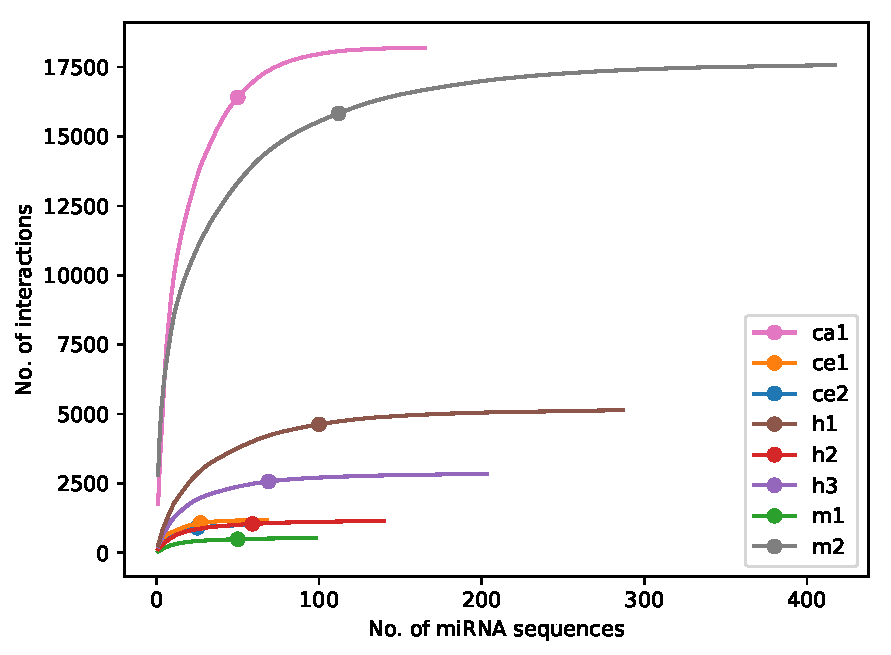
\includegraphics[width=\textwidth]{figures/1_mirna_dist.pdf}
      \label{fig:datasetplot}
      \caption*{Each curve corresponds to the cumulative sum of one of the datasets, where the bold points indicate the minimum number of unique miRNA sequences needed to represent 90\% of the interactions within a dataset. The height of a curve represents the size of the dataset, and the width of a curve represents the number of unique miRNA sequences that comprise the dataset.}
      \end{figure}

\subsection{Seed types and base-pairing density}
We classified the interactions (i.e., the corresponding duplexes formed by the miRNA and the target site) based on two parameters: seed type (canonical or non-canonical, see methods) and base-pairing density (number of base-pairs (bp) within the duplex: low with less than 11bp, medium with 11-16bp and high with more than 16bp). We defined 6 classes based on combinations of seed type and base-pairing density and assigned each interaction to the appropriate class (Figure \ref{fig:seed_type_pos}). As can be seen in the figure, the datasets are rich and diverse and include all the combinations of seed type and base-pairing density.
Nevertheless, two observations stand out: 
(1) In terms of seed type, the majority of the interactions are non-canonical (48-70\%); and (2) for both classes of seed types,  the majority of the interactions have medium and high base-pairing density, while the low base-pairing density interactions comprise only a small portion of the datasets. Similar analysis for the negative interactions is shown in Figure \ref{fig:seed_type_neg}


\begin{figure}[h!]
  \caption{\textbf{Classification of the miRNA-target duplexes based on their base-pairing patterns}} 
    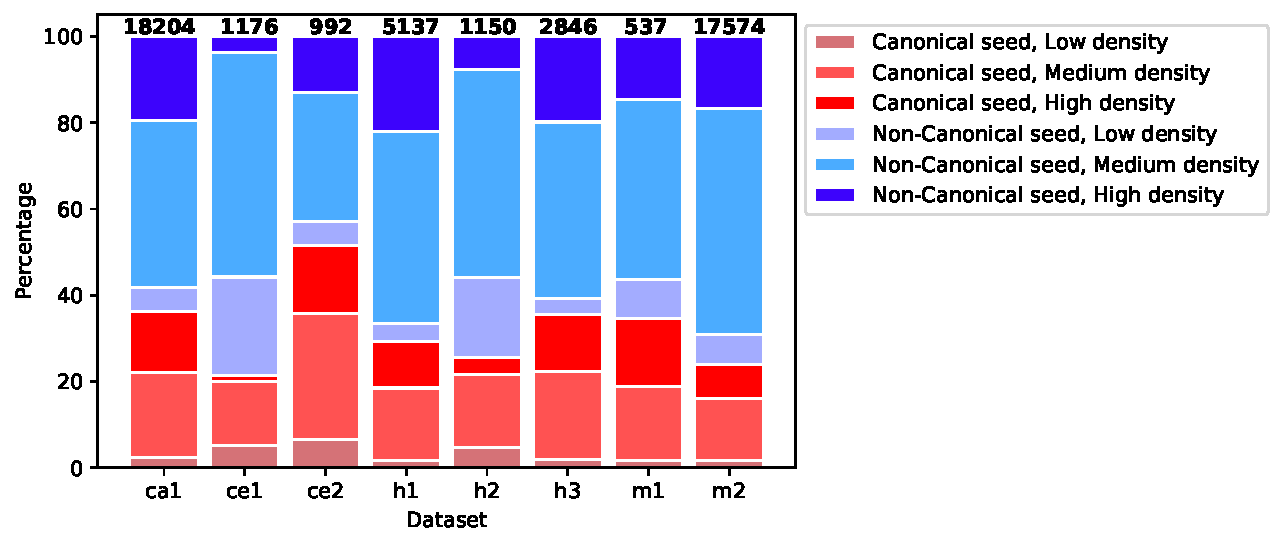
\includegraphics[width = 1\textwidth]{figures/2_seed_type_positive2.pdf}
      \label{fig:seed_type_pos}
      \caption*{Distribution of miRNA-target duplexes across 6 classes according to the seed type (canonical and non-canonical) and to the base-pairing density (low: less than 11bp, medium: 11-16bp and high: more than 16bp).}

      \end{figure}
      

\begin{figure}[h!]
 \centering
  \caption{\textbf{Classification of the negative miRNA-target duplexes based on their base-pairing patterns}}
    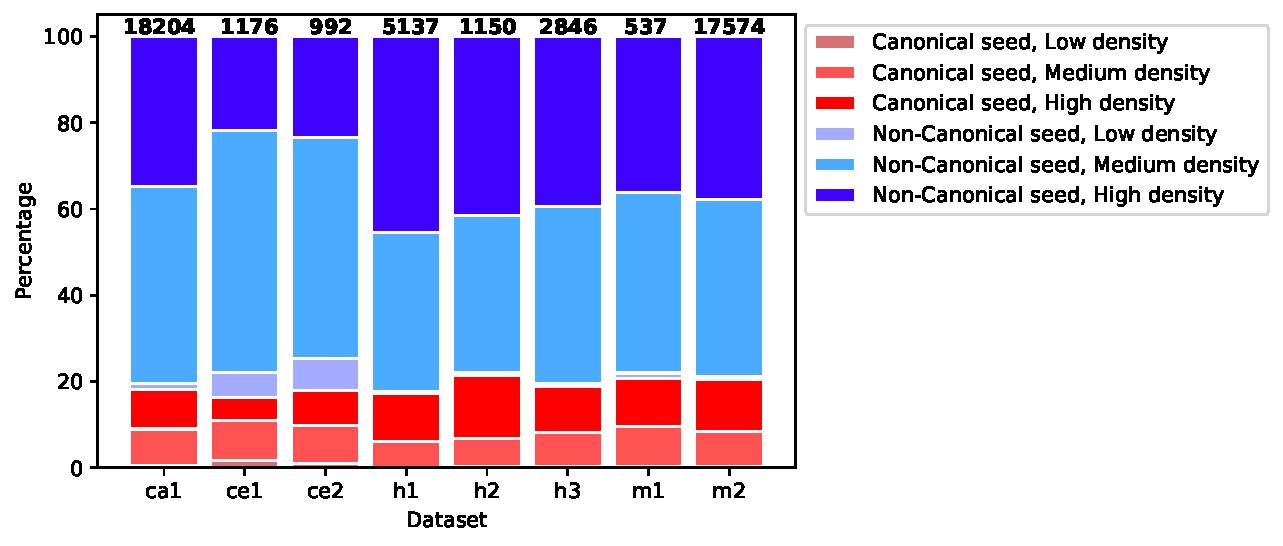
\includegraphics[width = 1\textwidth]{figures/seed_type_negative2.pdf}
      \label{fig:seed_type_neg}
      \caption*{Distribution of miRNA-target duplexes across 6 classes according to the seed type (canonical and non-canonical) and to the base-pairing density (low: less than 11bp, medium: 11-16bp and high: more than 16bp).}
      \end{figure}




\section{Intra-dataset analysis} \label{nameref:indataset}
In this section, we evaluated the performance of machine-learning-based binary classifiers to correctly classify positive and negative miRNA-target interactions within the same dataset. 
We first conducted a set of experiments with different types of commonly used machine learning classifiers. Then, we performed an in-depth analysis of the best performing classifier, by measuring different performance metrics and by estimating feature importance.

\subsection{Evaluation of different machine learning methods} \label{sec:evaluation_different_ML}
For each dataset, we generated 20 training-testing splits of the data using a stratified random split algorithm. This split algorithm ensures that each miRNA appears in the training and the testing sets at the same proportion as in the original dataset.
We then trained 6 widely used classifiers on the 20 training sets of each dataset and measured their performance in the classification of their respective testing sets. We calculated the mean and the standard deviation values of the classification accuracy as shown in Table \ref{tab:self_summary}. Notably, XGBoost classifier achieved the best results across all datasets, with accuracy scores ranging from 0.82 to 0.94, with the following order of performance from low to high: \textit{h1},  \textit{h3},  \textit{m1}, \textit{ce1}, \textit{ce2}, \textit{m2}, \textit{h2}, \textit{ca1}. We did not observe any bias in the ordering of the organisms in the list.   
We compared our results to previous machine learning-based approaches that were trained and tested on the human CLASH dataset designated as \textit{h1} in Table \ref{tbl:dataset_description}. The accuracy achieved by our classifiers on this dataset is comparable to the ones reported by previous studies (Table \ref{tab:existingmethods}). 


\begin{table}[h!]
\caption{Intra-dataset classification accuracy of different machine learning methods}
\label{tab:self_summary}
\begin{tabular}{|l|l|l|l|l|l|l|}
\hline
Dataset & XGBoost & RF & KNN & SGD & SVM & LR \\ \hline
ca1                               & \begin{tabular}[c]{@{}l@{}}0.937 \\ (0.002)\end{tabular} & \begin{tabular}[c]{@{}l@{}}0.885 \\ (0.004)\end{tabular} & \begin{tabular}[c]{@{}l@{}}0.828 \\ (0.003)\end{tabular} & \begin{tabular}[c]{@{}l@{}}0.797 \\ (0.033)\end{tabular} & \begin{tabular}[c]{@{}l@{}}0.895 \\ (0.003)\end{tabular} & \begin{tabular}[c]{@{}l@{}}0.836 \\ (0.004)\end{tabular} \\ \hline
ce1                               & \begin{tabular}[c]{@{}l@{}}0.889 \\ (0.014)\end{tabular} & \begin{tabular}[c]{@{}l@{}}0.833 \\ (0.019)\end{tabular} & \begin{tabular}[c]{@{}l@{}}0.768 \\ (0.019)\end{tabular} & \begin{tabular}[c]{@{}l@{}}0.798 \\ (0.045)\end{tabular} & \begin{tabular}[c]{@{}l@{}}0.841 \\ (0.015)\end{tabular} & \begin{tabular}[c]{@{}l@{}}0.843 \\ (0.014)\end{tabular} \\ \hline
ce2                               & \begin{tabular}[c]{@{}l@{}}0.891 \\ (0.016)\end{tabular} & \begin{tabular}[c]{@{}l@{}}0.858 \\ (0.018)\end{tabular} & \begin{tabular}[c]{@{}l@{}}0.768 \\ (0.019)\end{tabular} & \begin{tabular}[c]{@{}l@{}}0.819 \\ (0.034)\end{tabular} & \begin{tabular}[c]{@{}l@{}}0.862 \\ (0.012)\end{tabular} & \begin{tabular}[c]{@{}l@{}}0.847 \\ (0.016)\end{tabular} \\ \hline
h1                                & \begin{tabular}[c]{@{}l@{}}0.824 \\ (0.007)\end{tabular} & \begin{tabular}[c]{@{}l@{}}0.769 \\ (0.008)\end{tabular} & \begin{tabular}[c]{@{}l@{}}0.731 \\ (0.007)\end{tabular} & \begin{tabular}[c]{@{}l@{}}0.746 \\ (0.011)\end{tabular} & \begin{tabular}[c]{@{}l@{}}0.795 \\ (0.007)\end{tabular} & \begin{tabular}[c]{@{}l@{}}0.770 \\ (0.007)\end{tabular} \\ \hline
h2                                & \begin{tabular}[c]{@{}l@{}}0.904 \\ (0.007)\end{tabular} & \begin{tabular}[c]{@{}l@{}}0.869 \\ (0.011)\end{tabular} & \begin{tabular}[c]{@{}l@{}}0.857 \\ (0.009)\end{tabular} & \begin{tabular}[c]{@{}l@{}}0.860 \\ (0.03)\end{tabular}  & \begin{tabular}[c]{@{}l@{}}0.879 \\ (0.009)\end{tabular} & \begin{tabular}[c]{@{}l@{}}0.892 \\ (0.009)\end{tabular} \\ \hline
h3                                & \begin{tabular}[c]{@{}l@{}}0.835 \\ (0.007)\end{tabular} & \begin{tabular}[c]{@{}l@{}}0.769 \\ (0.009)\end{tabular} & \begin{tabular}[c]{@{}l@{}}0.744 \\ (0.009)\end{tabular} & \begin{tabular}[c]{@{}l@{}}0.752 \\ (0.034)\end{tabular} & \begin{tabular}[c]{@{}l@{}}0.805 \\ (0.007)\end{tabular} & \begin{tabular}[c]{@{}l@{}}0.795 \\ (0.010)\end{tabular} \\ \hline
m1                                & \begin{tabular}[c]{@{}l@{}}0.847 \\ (0.015)\end{tabular} & \begin{tabular}[c]{@{}l@{}}0.795\\ (0.016)\end{tabular}  & \begin{tabular}[c]{@{}l@{}}0.758 \\ (0.022)\end{tabular} & \begin{tabular}[c]{@{}l@{}}0.760 \\ (0.038)\end{tabular} & \begin{tabular}[c]{@{}l@{}}0.819 \\ (0.019)\end{tabular} & \begin{tabular}[c]{@{}l@{}}0.800 \\ (0.019)\end{tabular} \\ \hline
m2                                & \begin{tabular}[c]{@{}l@{}}0.900 \\ (0.004)\end{tabular} & \begin{tabular}[c]{@{}l@{}}0.826 \\ (0.004)\end{tabular} & \begin{tabular}[c]{@{}l@{}}0.797 \\ (0.004)\end{tabular} & \begin{tabular}[c]{@{}l@{}}0.798 \\ (0.017)\end{tabular} & \begin{tabular}[c]{@{}l@{}}0.873\\ (0.004)\end{tabular}  & \begin{tabular}[c]{@{}l@{}}0.833 \\ (0.004)\end{tabular} \\ \hline
\end{tabular}
\caption*{The cells contain the mean and the standard deviation (in brackets) values of the accuracy results acquired from 20 models that were trained and evaluated on different training-testing dataset splits}
\end{table}



\subsection{In-depth analysis of the XGBoost performance}
We next sought to perform an in-depth performance analysis for the XGBoost classifier since it achieved the highest accuracy across all datasets. Therefore, we calculated 5 additional commonly used performance metrics. 
The area under the curve (AUC) is a performance measurement for classification problems at different threshold settings. It provides information on the capability of a model to differentiate between classes. AUC values range from 0 to 1, where a model with perfect predictions achieves AUC of 1. 
True positive rate (TPR) and true negative rate (TNR) are the percentages of actual positive or negative results that are correctly identified.  For ideal classifiers, these metrics are close to 1. The Matthews correlation coefficient (MCC) is used as a measure of the quality of classifications. A coefficient of +1 represents a perfect prediction, 0 an average random prediction, and -1 an inverse prediction. 
The F1 score is an average of two metrics: precision (proportion of positive classification which was correct) and recall (proportion of positives that were correctly classified). The F1 score reaches its best value at 1 and its worst score at 0. 

We observed that the values for all datasets are similar and relatively high. Table \ref{tab:measurementinfo} summarises the performance metrics of the XGBoost classifiers for each dataset. As before, we calculated the mean scores and the standard deviation values of the metrics across 20 training-testing data splits. The average metrics scores ranged as follows: AUC score ranged in 0.91-0.98, TPR and TNR ranged in 0.82-0.91, MCC coefficient ranged in 0.65-0.87, and F1 score ranged in 0.82-0.94. In accordance with the accuracy metric previously calculated, these metrics indicate that all 8 XGBoost classifiers (corresponding to each dataset) are accurate, balanced, and precise. 


\begin{table}[h!]
\caption{XGBoost performance measurements}
\label{tab:measurementinfo}
  \begin{threeparttable}

\begin{tabular}{|l|l|l|l|l|l|l|}
\hline
 Dataset   & AUC \tnote{a}     & ACC \tnote{b}           & TPR \tnote{c}          & TNR \tnote{d}          & MCC \tnote{e}          & F1 score      \\ \hline
ca1 & \begin{tabular}[c]{@{}l@{}} 0.983 \\ (0.001)\end{tabular} & \begin{tabular}[c]{@{}l@{}} 0.937 \\ (0.002)\end{tabular} & \begin{tabular}[c]{@{}l@{}} 0.932 \\ (0.004)\end{tabular} & \begin{tabular}[c]{@{}l@{}} 0.943 \\ (0.004)\end{tabular} & \begin{tabular}[c]{@{}l@{}} 0.874 \\ (0.004)\end{tabular} & \begin{tabular}[c]{@{}l@{}} 0.937 \\ (0.002)\end{tabular} \\ \hline
ce1 & \begin{tabular}[c]{@{}l@{}} 0.955 \\ (0.009)\end{tabular} & \begin{tabular}[c]{@{}l@{}} 0.889 \\ (0.014)\end{tabular} & \begin{tabular}[c]{@{}l@{}} 0.89 \\ (0.018)\end{tabular}  & \begin{tabular}[c]{@{}l@{}} 0.889 \\ (0.014)\end{tabular} & \begin{tabular}[c]{@{}l@{}} 0.779 \\ (0.028)\end{tabular} & \begin{tabular}[c]{@{}l@{}} 0.89 \\ (0.014)\end{tabular}  \\ \hline
ce2 & \begin{tabular}[c]{@{}l@{}} 0.958 \\ (0.012)\end{tabular} & \begin{tabular}[c]{@{}l@{}} 0.891 \\ (0.016)\end{tabular} & \begin{tabular}[c]{@{}l@{}} 0.884 \\ (0.02)\end{tabular}  & \begin{tabular}[c]{@{}l@{}} 0.899 \\ (0.019)\end{tabular} & \begin{tabular}[c]{@{}l@{}} 0.783 \\ (0.032)\end{tabular} & \begin{tabular}[c]{@{}l@{}} 0.89 \\ (0.017)\end{tabular}  \\ \hline
h1  & \begin{tabular}[c]{@{}l@{}} 0.908 \\ (0.006)\end{tabular} & \begin{tabular}[c]{@{}l@{}} 0.824 \\ (0.007)\end{tabular} & \begin{tabular}[c]{@{}l@{}} 0.816 \\ (0.008)\end{tabular} & \begin{tabular}[c]{@{}l@{}} 0.833 \\ (0.008)\end{tabular} & \begin{tabular}[c]{@{}l@{}} 0.649 \\ (0.014)\end{tabular} & \begin{tabular}[c]{@{}l@{}} 0.822 \\ (0.007)\end{tabular} \\ \hline
h2  & \begin{tabular}[c]{@{}l@{}} 0.972 \\ (0.003)\end{tabular} & \begin{tabular}[c]{@{}l@{}} 0.904 \\ (0.007)\end{tabular} & \begin{tabular}[c]{@{}l@{}} 0.886 \\ (0.012)\end{tabular} & \begin{tabular}[c]{@{}l@{}} 0.924 \\ (0.011)\end{tabular} & \begin{tabular}[c]{@{}l@{}} 0.809 \\ (0.014)\end{tabular} & \begin{tabular}[c]{@{}l@{}} 0.902 \\ (0.007)\end{tabular} \\ \hline
h3  & \begin{tabular}[c]{@{}l@{}} 0.914 \\ (0.004)\end{tabular} & \begin{tabular}[c]{@{}l@{}} 0.835 \\ (0.007)\end{tabular} & \begin{tabular}[c]{@{}l@{}} 0.823 \\ (0.011)\end{tabular} & \begin{tabular}[c]{@{}l@{}} 0.849 \\ (0.009)\end{tabular} & \begin{tabular}[c]{@{}l@{}} 0.671 \\ (0.014)\end{tabular} & \begin{tabular}[c]{@{}l@{}} 0.832 \\ (0.008)\end{tabular} \\ \hline
m1  & \begin{tabular}[c]{@{}l@{}} 0.914 \\ (0.007)\end{tabular} & \begin{tabular}[c]{@{}l@{}} 0.847 \\ (0.015)\end{tabular} & \begin{tabular}[c]{@{}l@{}} 0.834 \\ (0.014)\end{tabular} & \begin{tabular}[c]{@{}l@{}} 0.862 \\ (0.024)\end{tabular} & \begin{tabular}[c]{@{}l@{}} 0.695 \\ (0.031)\end{tabular} & \begin{tabular}[c]{@{}l@{}} 0.844 \\ (0.014)\end{tabular} \\ \hline
m2  & \begin{tabular}[c]{@{}l@{}} 0.963 \\ (0.002)\end{tabular} & \begin{tabular}[c]{@{}l@{}} 0.9 \\ (0.004)\end{tabular}   & \begin{tabular}[c]{@{}l@{}} 0.891 \\ (0.003)\end{tabular} & \begin{tabular}[c]{@{}l@{}} 0.909 \\ (0.005)\end{tabular} & \begin{tabular}[c]{@{}l@{}} 0.8 \\ (0.008)\end{tabular}   & \begin{tabular}[c]{@{}l@{}} 0.899 \\ (0.004)\end{tabular} \\ \hline
\end{tabular}
\begin{tablenotes}\footnotesize
\item[a] Area Under the Receiver Operating Characteristic Curve
\item[b] Overall accuracy
\item[c] True Positive Rate (Sensitivity)
\item[d] True Negative Rate (Specificity)
\item[e] Matthews correlation coefficient
% \item[f] also (F1 score or F-measure)
\end{tablenotes}
\end{threeparttable}
\caption*{The cells contain the mean scores and the standard deviation (in brackets) values acquired from 20 models that were trained and evaluated on different training-testing dataset splits.}
\end{table}



\subsection{Random split control}
In the above analysis, the splitting of the dataset into the training and testing sets was done in a way that preserves the miRNA distribution in both sets (stratified split). To assess how this type of split affects the classifier performance, we repeated the analysis with the XGBoost classifier, but this time used a random split strategy (control split) to generate the training and the testing sets. Our results showed that there is almost no difference between the results achieved with the stratified and the control split methods. The accuracy results for the control splits are found in Table \ref{tab:randomsplitacc}


\begin{table}[h!]
\caption{Classification accuracy of xGBoost when applied to random (control) training-testing dataset splits}
\label{tab:randomsplitacc}
\centering
\begin{tabular}{|l|l|}
\hline
\textbf{Dataset} & \textbf{Accuracy}      \\ \hline
ca1   & 0.938 (0.004) \\ \hline
ce1 & 0.891 (0.013) \\ \hline
ce2 & 0.89 0(0.012) \\ \hline
h1    & 0.832 (0.006) \\ \hline
h2    & 0.920 (0.013) \\ \hline
h3    & 0.849 (0.008) \\ \hline
m1    & 0.848 (0.011) \\ \hline
m2    & 0.897 (0.006) \\ \hline
\end{tabular}
\bigbreak
\caption*{The cells contain the mean and the standard deviation values (in brackets) acquired from 5 models that were trained and evaluated on different random dataset splits.}
\end{table}



\subsection{Top important features of each dataset}
We used 490 features to describe the interactions. We next sought to identify the top important features of each dataset, their relative scores, and the degree of overlap of the top features between different datasets. XGBoost classifier reports a list of five feature importance metrics: weight, gain, cover, total gain, and total cover. We extracted the 5 metrics for all the 20 training-testing splits of each dataset and calculated their mean and standard deviation. 
For further analysis, we chose the gain metric, which reflects the contribution of each feature to the model. For each dataset, we sorted the features in descending order, based on their mean gain score. The plots of the feature importance curves for all datasets are shown in Figure \ref{fig:feature_importance}.
Figure \ref{fig:feature_importance}a reveals that the gain score is decaying very fast. The 6 top features are significantly stronger relative to the rest (Figure \ref{fig:feature_importance}b). We thus extracted the top 6 features from each dataset, along with their scaled gain score (see methods), into a unified list. The unified list consisted of a total of 16 features (out of the maximum length of 48), indicating that there are many shared features among the datasets. Table \ref{tab:feature_importance} shows the features ordered by their mean gain across all datasets and the top six features of each dataset are marked with a star. As can be seen in the table, there are at least 3 features common to each dataset pair. In addition, only a small number of features belong to a single dataset, indicating that the features in the unified list may well represent all 8 datasets.
Notably, features related to the seed region (marked as bold in the table), comprise half of the features in the list. This finding emphasizes the role of the seed region in the formation of miRNA-mRNA interactions.


\begin{figure}[h!]
    \centering
     \caption{\textbf{Datasets' feature importance plot based on gain score}}
    \subfloat[Full view of datasets' feature importance]{{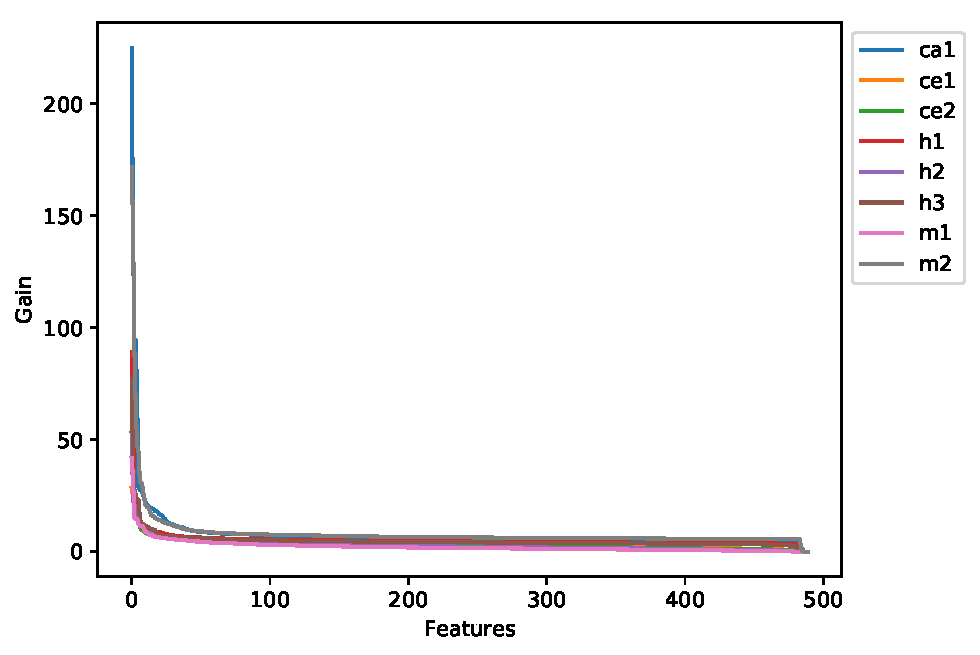
\includegraphics[width=5cm]{figures/3a_feature_importance_full.pdf} }}%
    \qquad
    \subfloat[View of the top 20 features score]{{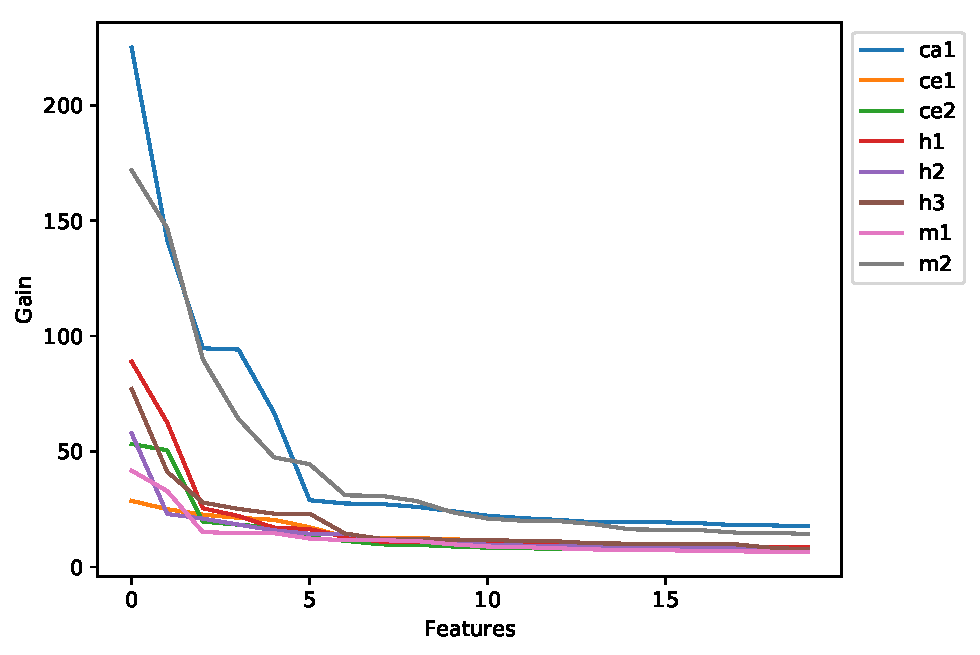
\includegraphics[width=5cm]{figures/3b_feature_importance_zoom.pdf} }}%
    \caption*{The features are sorted in descending order from the top feature (highest gain) to lowest. (a) A full view of the gain plot emphasizes the gain decay.  (b) A zoomed view, focused on the top 20 features.}%
    \label{fig:feature_importance}%
\end{figure}



\begin{table}[h!]
\caption{Feature importance}
\label{tab:feature_importance}
 \begin{threeparttable}
                     \resizebox{\textwidth}{!}{%

\begin{tabular}{|l|l|l|l|l|l|l|l|l|l|}
\hline
\textbf{Feature/Dataset}                          & \textbf{ca1} & \textbf{ce1} & \textbf{ce2} & \textbf{h1} & \textbf{h2} & \textbf{h3} & \textbf{m1} & \textbf{m2} & \textbf{mean} \\ \hline
\textbf{Number of GU bp within the seed\tnote{n}}              & 100\tnote{*}          & 87\tnote{*}           & 95\tnote{*}           & 29\tnote{*}          & 40\tnote{*}          & 100\tnote{*}         & 28          & 100\tnote{*}         & 72            \\ \hline
\textbf{bp in the 1st nt of the seed\tnote{b}}                    & 63\tnote{*}           & 79\tnote{*}           & 34\tnote{*}           & 70\tnote{*}          & 25\tnote{*}          & 30\tnote{*}          & 27          & 85\tnote{*}          & 52            \\ \hline
Number of GU bp within the site\tnote{n}                      & 42\tnote{*}           & 71\tnote{*}           & 32\tnote{*}           & 100\tnote{*}         & 19          & 53\tnote{*}          & 35\tnote{*}          & 28\tnote{*}          & 48            \\ \hline
Proportion of G in mRNA at the site region\tnote{n}                             & 12           & 74\tnote{*}           & 12           & 12          & 36\tnote{*}          & 33\tnote{*}          & 100\tnote{*}         & 37\tnote{*}          & 39            \\ \hline
Duplex minimum free energy\tnote{n}                               & 13\tnote{*}           & 45           & 11           & 10          & 100\tnote{*}         & 19          & 35\tnote{*}          & 52\tnote{*}          & 36            \\ \hline
\textbf{Number of bp at location 2-7\tnote{n}} & 42\tnote{*}           & 33           & 100\tnote{*}          & 12          & 18          & 36\tnote{*}          & 13          & 18          & 34            \\ \hline
Proportion of GG in mRNA at the site region\tnote{n}                            & 30\tnote{*}           & 21           & 10           & 12          & 7           & 30\tnote{*}          & 79\tnote{*}          & 26\tnote{*}          & 27            \\ \hline
\textbf{bp in the 4th nt of the seed\tnote{b}}                    & 8            & 100\tnote{*}          & 21           & 10          & 11          & 16          & 2           & 12          & 22            \\ \hline
Number of bulges outside the seed\tnote{n}                 & 3            & 60\tnote{*}           & 6            & 25\tnote{*}          & 32\tnote{*}          & 9           & 9           & 8           & 19            \\ \hline
\textbf{bp in the 2nd nt of the seed\tnote{b}}                    & 8            & 42           & 37\tnote{*}           & 7           & 11          & 13          & 15          & 6           & 17            \\ \hline
\textbf{bp in the 5th nt of the seed\tnote{b}}                    & 12           & 27           & 14           & 14          & 6           & 15          & 29\tnote{*}          & 12          & 16            \\ \hline
\textbf{Number of GC bp within the seed\tnote{n}}              & 7            & 22           & 24\tnote{*}           & 18\tnote{*}          & 12          & 13          & 11          & 12          & 15            \\ \hline
Number of GC bp outside the seed\tnote{n}                         & 4            & 27           & 11           & 10          & 27\tnote{*}          & 8           & 6           & 5           & 12            \\ \hline
Accessibility (nt=21, len=10)\tnote{n}                                    & 9            & 19           & 7            & 6           & 25          & 7           & 12          & 7           & 11            \\ \hline
minimum free energy of the target site + 50nt flanking regions\tnote{n}            & 8            & 11           & 6            & 7           & 8           & 11          & 36\tnote{*}          & 6           & 11            \\ \hline
\textbf{Number of mismatches inside the seed\tnote{n}}    & 4            & 3            & 15           & 19\tnote{*}          & 0           & 13          & 2           & 9           & 8             \\ \hline
\end{tabular}}
\begin{tablenotes}\footnotesize
\item[*] Belongs to the top 6 features of the dataset
\item[b] Boolean feature
\item[n] Numeric feature

\end{tablenotes}
 \end{threeparttable}
 \caption*{The table shows 16 features representing the union of the top 6 features of each dataset, along with their gain values which were computed by XGBoost. The features are ordered by their mean gain, scaled to the range of (0, 100), across all datasets. For the unscaled version of the table, see Table \ref{tab:feature_importance_unscaled}}
\end{table}


\begin{table}[h!]
\caption{Feature importance}
\label{tab:feature_importance_unscaled}
\centering
                    \resizebox{\textwidth}{!}{%

\begin{tabular}{|l|l|l|l|l|l|l|l|l|l|}
\hline
\textbf{Feature/Dataset}                                   & \textbf{ca1} & \textbf{ce1} & \textbf{ce2} & \textbf{h1} & \textbf{h2} & \textbf{h3} & \textbf{m1} & \textbf{m2} & \textbf{mean} \\ \hline
 \textbf{Number of GU bp within the seed}                 & 225          & 25           & 51           & 25          & 23          & 77          & 12          & 172         & 76            \\ \hline
 \textbf{bp in the 1st nt of the seed}                       & 142          & 23           & 18           & 63          & 14          & 23          & 11          & 147         & 55            \\ \hline
Number of GU bp within the site                               & 94           & 20           & 17           & 89          & 11          & 41          & 15          & 47          & 42            \\ \hline
\textbf{Number of bp at location 2-7} & 95           & 9            & 53           & 11          & 10          & 28          & 6           & 31          & 30            \\ \hline
Duplex minimum free energy                                        & 29           & 13           & 6            & 9           & 58          & 14          & 15          & 90          & 29            \\ \hline
Proportion of G in mRNA at the site region                                      & 26           & 21           & 6            & 10          & 21          & 25          & 42          & 64          & 27            \\ \hline
Proportion of GG in mRNA at the site region                                     & 67           & 6            & 5            & 11          & 4           & 23          & 33          & 45          & 24            \\ \hline
\textbf{bp in the 4th nt of the seed}                    & 19           & 29           & 11           & 9           & 6           & 12          & 1           & 21          & 13            \\ \hline
\textbf{bp in the 5th nt of the seed}                    & 27           & 8            & 8            & 13          & 3           & 12          & 12          & 20          & 13            \\ \hline
Number of bulges outside the seed                          & 7            & 17           & 3            & 22          & 18          & 7           & 4           & 14          & 12            \\ \hline
\textbf{Number of GC bp within the seed}              & 15           & 6            & 13           & 16          & 7           & 10          & 4           & 20          & 11            \\ \hline
\textbf{bp in the 2nd nt of the seed}                    & 18           & 12           & 20           & 6           & 6           & 10          & 6           & 10          & 11            \\ \hline
Accessibility (nt=21, len=10)                                             & 19           & 5            & 4            & 6           & 14          & 6           & 5           & 11          & 9             \\ \hline
minimum free energy of the target site + 50nt flanking regions                     & 18           & 3            & 3            & 6           & 5           & 8           & 15          & 10          & 8             \\ \hline
Number of GC bp outside the seed                                 & 8            & 8            & 6            & 9           & 16          & 6           & 3           & 8           & 8             \\ \hline
\textbf{Number of mismatches inside the seed}    & 10           & 1            & 8            & 17          & 0           & 10          & 1           & 16          & 8             \\ \hline
\end{tabular}}
\bigbreak
\caption*{The table shows 16 features representing the union of the top 6 features of each dataset, along with their gain values which were computed by XGBoost. The features are ordered by their mean gain across all datasets. This is an unscaled version of Table 6.}
\end{table}







\section{Cross-dataset analysis}
In the previous section, we trained, optimized, and evaluated the performance of a dedicated classifier for each dataset. Next, we examined the relationships between datasets. To that end, we first used a statistical measure to calculate the distance between the datasets. Second, we visualized the datasets based on the unified list of the 16 most important features that were found above. Finally, we evaluated the performance of each dataset specific classifier to properly classify interactions in the other datasets.

\subsection{Kullback–Leibler divergence}
We hypothesized that a pair of datasets, with similar characteristics, might achieve better results in classifying the interactions of each other. We thus looked for a measure to assess the level of similarity of a pair of datasets, that will take into account the directionality of the classification task: classifier is trained on one dataset (source) and is applied to classify a second dataset (target).
We chose the asymmetric measure Kullback–Leibler (KL) divergence which measures how the target's probability distribution is different from the probability distribution of the source. KL divergence has its origins in information theory which deals with the quantification of the amount of information in a given data. KL divergence is widely used to assess the approximation of samples that come from one distribution by samples that come from another distribution. The KL divergence measures the information loss in the approximation. It is typically used to measure the information loss in a case when a simpler distribution (such as a Uniform or Gaussian distribution) approximates experimental data.

Similarly, we used the KL divergence to measure the pairwise information loss between every two datasets which will later be used as training and testing sets in the analysis described below. For each pair, we calculated the divergence that can be interpreted as the amount of information lost when the training set represents the testing set. The calculation is done based on the datasets' miRNA seed family distribution (see methods).

Figure \ref{fig:divergence} shows the divergence between all dataset pairs. The divergence of a dataset with itself is zero, and the divergence scores between datasets within the same organisms are usually lower than the divergence scores between different organisms. Notably, the divergence scores between \textit{C. elegans} datasets, both as targets and as sources, and the other datasets are significantly higher (range in 5-8.1) than the divergence scores between other pairs (range in 1.2-3.8), indicating that seed distributions of other organisms poorly represent the \textit{C. elegans} datasets and vice versa. The asymmetry of the KL measure can be observed, for example, for the pair \textit{(h1,h3)}, for which \textit{KL(target=h3 $||$ source=h1)=1.6} and the  \textit{KL(h1 $||$ h3)=2.1}. Intuitively, this means that dataset \textit{h1} better approximates dataset \textit{h3} and there is less information loss than in the vice-versa case.


\begin{figure}[h!]
  \caption{\textbf{Kullback–Leibler (KL) divergence of all dataset pairs}}
      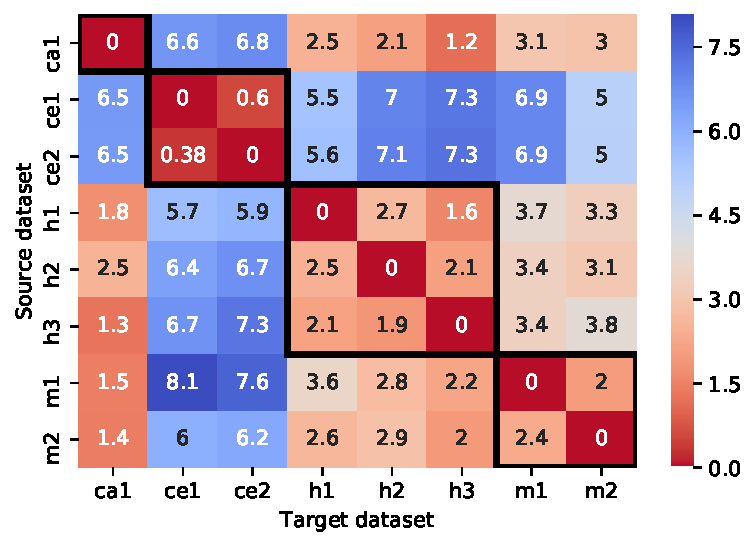
\includegraphics[width = 1\textwidth]{figures/4_divergence_reverse.pdf}
      \label{fig:divergence}
      \caption*{Each cell \textit{(i,j)} represents the divergence from  a source datasets \textit{i} to a target dataset \textit{j} (KL(j $||$ i)), based on their miRNA seed family distributions. The black frames surround the results of dataset pairs originating from the same organism.}
      \end{figure}


\subsection{Dataset visualization}
Visualization is an important step in the analysis of high-throughput biological data and can assist in revealing hidden phenomena. However, visualization is challenging when the data is represented by a large number of features. The dimensionality reduction algorithm enables the representation of the data in a 2-dimension scatter plot and facilitates the inspection of the data visually. To visualize the datasets in two dimensions, we first extracted for each dataset the unified list of 16 top features found above (see Table \ref{tab:feature_importance}) and then performed a dimensional reduction using the PCA technique. The results are shown in Figure \ref{fig:feature_pca}.

Figure \ref{fig:feature_pca} reiterates the fact that there are big differences in the sizes of the datasets, reflected in the density of the graphs. For example, the size of the human dataset \textit{h1} is more than twice the size of the datasets \textit{h2} and \textit{h3}, and indeed, its graph is denser. In addition, there are notable differences in the 2-dimensional space spanned by each dataset: while the datasets \textit{ca1}, \textit{h1}, \textit{h3}, \textit{m2} are spread in the whole area, \textit{C. elegans} datasets (\textit{ce1}, \textit{ce2}) and datasets composed of endogenously ligated chimeras from a mixture of experiments (\textit{h2}, \textit{m1}) are concentrated in a narrower part of the area.


\begin{figure}[h!]
  \caption{\textbf{Visualization of the datasets in 2D}} 
       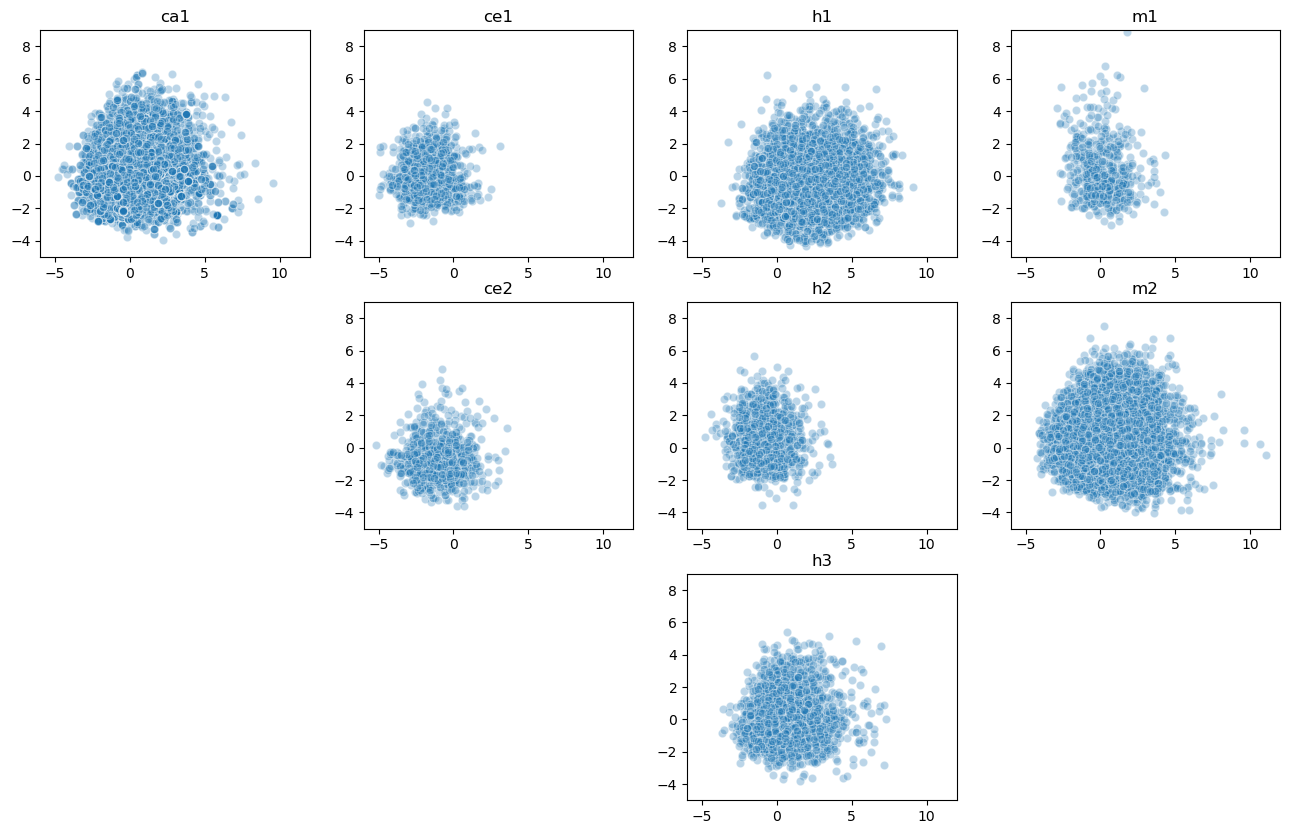
\includegraphics[width = 1\textwidth]{figures/5_unite_features_pca_resample_scale=True_all.png}
      \label{fig:feature_pca}
      \caption*{Each point represents a single interaction after a dimensional reduction of its features' space using PCA. X and Y axes are the first and the second components of the PCA, respectively.}
      \end{figure}

  


\subsection{Classification performance between datasets}
We evaluated the performance of cross dataset miRNA-target predictions, i.e., the performance of a classifier when applied to interactions from datasets different from the one it was trained on.
We examined all possible 56 combinations, considering each dataset both as a training and as a testing set. 
For each dataset, we loaded the 20 XGBoost classifiers that we trained in section \nameref{nameref:indataset} and used them to classify the rest 7 datasets. Figure \ref{fig:crossdataset} shows for every pair of datasets the mean classification accuracy over the 20 tests (for standard deviation values, see Table \ref{tab:diff})

Inspection of the results (excluding the diagonal) reveals that there is a variability in the classification performance among the pairs, ranging from random, slightly above 0.5, to 0.91. The accuracy matrix is not symmetric, i.e., a pair where a dataset \textit{i} serves as a training set and a dataset \textit{j} serves as a testing set, achieves a different performance than a swapped pair. Pairs of datasets originating from the same organism (surrounded by black boxes in Figure \ref{fig:crossdataset}) generally achieved higher accuracy than pairs from mixed organisms. Intriguingly, the human pairs \textit{(h2,h1)}, \textit{(h2,h3), \textit{(h3,h1)}} achieved a relatively low accuracy score. The low performance of these pairs could be potentially explained by the differences in the diversity of the datasets. In particular, the dataset \textit{h2} is smaller and less diverse then the datasets \textit{h1,h3} (Figure \ref{fig:feature_pca}), and thus a model that uses it as a training set achieves lower performance. In most of the cases, the KL divergence results coincide with the accuracy results. For example, for the pair \textit{(h1,h3)}, the \textit{KL(h3 $||$ h1)=1.6 $<$ KL(h3 $||$ h1)=2.1} while \textit{ACC(train=h1, test=h3)=0.79 $>$ ACC(h3,h1)=0.69}, demonstrating that the dataset \textit{h1} better represents the dataset \textit{h3} and as such achieved better accuracy results than vice versa. Interestingly, the \textit{KL(h2 $||$ h1)=2.5 $\approx$ KL(h1 $||$ h2)=2.7} however the \textit{ACC(h1,h2)=0.86 $>$ ACC(h2,h1)=0.58}. This indicates that there are additional factors that affect the ability to accurately classify miRNA-target interactions, such as the patterns of interactions that appear in them.

Pairs of datasets originating from different organisms, that included \textit{C. elegans} as either a training or a testing set achieved poor performance, which ranged from 0.56 to 0.78. As we previously saw, the divergence scores of these pairs are 2x-4x larger (range from 5 to 8) than the scores of the other pairs. This may indicate that the seed distributions of human, mouse and cattle datasets are not well represented by the seed distributions of \textit{C. elegans} datasets and vice versa. Other pairs of two organisms achieve much higher accuracy, reaching up to 0.91. The lowest accuracy in these mixed pairs was observed for pairs that contained \textit{h1} as a testing set. Notably, this dataset was used by previous methods (Table \ref{tab:toolsummary}) for training/testing purposes only, and has never been evaluated as an independent testing set. Additional factors that could influence the classification accuracy will be further discussed in the discussion section.

\begin{figure}[h!]
  \caption{\textbf{Cross-dataset classification results}}
      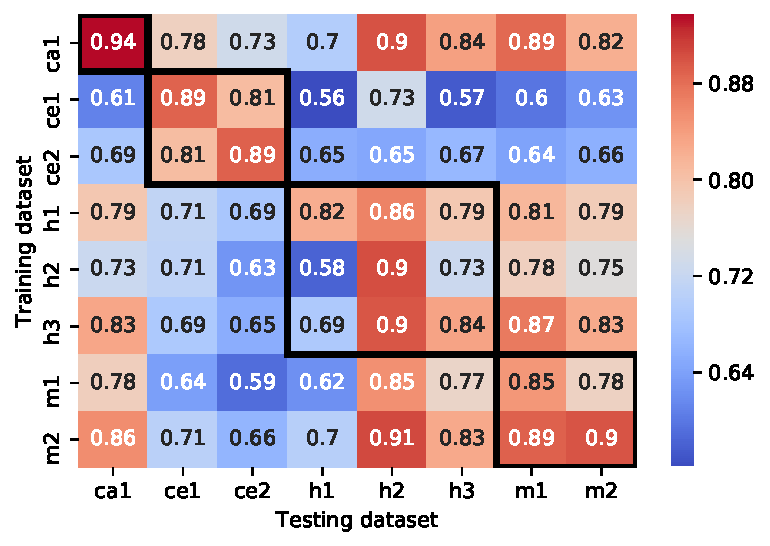
\includegraphics[width = 1\textwidth]{figures/6_diff_summary.pdf}
    \label{fig:crossdataset}
    \caption*{Each cell \textit{(i,j)} represents the mean accuracy of the 20 classifiers that were trained on dataset \textit{i} (in section \nameref{sec:evaluation_different_ML}) and tested on dataset \textit{j} (ACC(i, j)). The black frames surround the results of dataset pairs originating from the same organism. The accuracy results for pairs \textit{(i,i)}, were taken from section \nameref{nameref:indataset}. Note: The color scale of this figure is inverse to the scale used for KL-divergence plot in Figure \ref{fig:divergence}}
      \end{figure}




\begin{table}[h!]
\caption{\textbf{Cross-dataset classification results (complementary information to Figure \ref{fig:crossdataset})}}
\label{tab:diff}
\centering
\begin{tabular}{|l|l|l|l|l|l|l|l|l|}
\hline
    & ca1           & ce1           & ce2           & h1            & h2            & h3            & m1            & m2            \\ \hline
ca1 & \begin{tabular}[c]{@{}l@{}} 0.937 \\ (0.002)\end{tabular} & \begin{tabular}[c]{@{}l@{}} 0.779 \\ (0.005)\end{tabular} & \begin{tabular}[c]{@{}l@{}} 0.733 \\ (0.01)\end{tabular}  & \begin{tabular}[c]{@{}l@{}} 0.699 \\ (0.003)\end{tabular} & \begin{tabular}[c]{@{}l@{}} 0.902 \\ (0.002)\end{tabular} & \begin{tabular}[c]{@{}l@{}} 0.839 \\ (0.002)\end{tabular} & \begin{tabular}[c]{@{}l@{}} 0.885 \\ (0.006)\end{tabular} & \begin{tabular}[c]{@{}l@{}} 0.823 \\ (0.002)\end{tabular} \\ \hline
ce1 & \begin{tabular}[c]{@{}l@{}} 0.61 \\ (0.005)\end{tabular}  & \begin{tabular}[c]{@{}l@{}} 0.889 \\ (0.014)\end{tabular} & \begin{tabular}[c]{@{}l@{}} 0.809 \\ (0.011)\end{tabular} & \begin{tabular}[c]{@{}l@{}} 0.561 \\ (0.006)\end{tabular} & \begin{tabular}[c]{@{}l@{}} 0.732 \\ (0.009)\end{tabular} & \begin{tabular}[c]{@{}l@{}} 0.575 \\ (0.005)\end{tabular} & \begin{tabular}[c]{@{}l@{}} 0.598 \\ (0.008)\end{tabular} & \begin{tabular}[c]{@{}l@{}} 0.626 \\ (0.006)\end{tabular} \\ \hline
ce2 & \begin{tabular}[c]{@{}l@{}} 0.688 \\ (0.008)\end{tabular} & \begin{tabular}[c]{@{}l@{}} 0.806 \\ (0.007)\end{tabular} & \begin{tabular}[c]{@{}l@{}} 0.891 \\ (0.016)\end{tabular} & \begin{tabular}[c]{@{}l@{}} 0.654 \\ (0.008)\end{tabular} & \begin{tabular}[c]{@{}l@{}} 0.647 \\ (0.008)\end{tabular} & \begin{tabular}[c]{@{}l@{}} 0.667 \\ (0.008)\end{tabular} & \begin{tabular}[c]{@{}l@{}} 0.643 \\ (0.01)\end{tabular}  & \begin{tabular}[c]{@{}l@{}} 0.657 \\ (0.006)\end{tabular} \\ \hline
h1  & \begin{tabular}[c]{@{}l@{}} 0.794 \\ (0.005)\end{tabular} & \begin{tabular}[c]{@{}l@{}} 0.714 \\ (0.007)\end{tabular} & \begin{tabular}[c]{@{}l@{}} 0.686 \\ (0.011)\end{tabular} & \begin{tabular}[c]{@{}l@{}} 0.824 \\ (0.007)\end{tabular} & \begin{tabular}[c]{@{}l@{}} 0.864 \\ (0.006)\end{tabular} & \begin{tabular}[c]{@{}l@{}} 0.792 \\ (0.004)\end{tabular} & \begin{tabular}[c]{@{}l@{}} 0.815 \\ (0.008)\end{tabular} & \begin{tabular}[c]{@{}l@{}} 0.786 \\ (0.004)\end{tabular} \\ \hline
h2  & \begin{tabular}[c]{@{}l@{}} 0.725 \\ (0.004)\end{tabular} & \begin{tabular}[c]{@{}l@{}} 0.712 \\ (0.005)\end{tabular} & \begin{tabular}[c]{@{}l@{}} 0.628 \\ (0.007)\end{tabular} & \begin{tabular}[c]{@{}l@{}} 0.582 \\ (0.004)\end{tabular} & \begin{tabular}[c]{@{}l@{}} 0.904 \\ (0.007)\end{tabular} & \begin{tabular}[c]{@{}l@{}} 0.727 \\ (0.004)\end{tabular} & \begin{tabular}[c]{@{}l@{}} 0.78 \\ (0.008)\end{tabular}  & \begin{tabular}[c]{@{}l@{}} 0.753 \\ (0.005)\end{tabular} \\ \hline
h3  & \begin{tabular}[c]{@{}l@{}} 0.832 \\ (0.004)\end{tabular} & \begin{tabular}[c]{@{}l@{}} 0.691 \\ (0.005)\end{tabular} & \begin{tabular}[c]{@{}l@{}} 0.654 \\ (0.009)\end{tabular} & \begin{tabular}[c]{@{}l@{}} 0.693 \\ (0.006)\end{tabular} & \begin{tabular}[c]{@{}l@{}} 0.898 \\ (0.003)\end{tabular} & \begin{tabular}[c]{@{}l@{}} 0.835 \\ (0.007)\end{tabular} & \begin{tabular}[c]{@{}l@{}} 0.872 \\ (0.007)\end{tabular} & \begin{tabular}[c]{@{}l@{}} 0.828 \\ (0.003)\end{tabular} \\ \hline
m1  & \begin{tabular}[c]{@{}l@{}} 0.782 \\ (0.007)\end{tabular} & \begin{tabular}[c]{@{}l@{}} 0.638 \\ (0.01)\end{tabular}  & \begin{tabular}[c]{@{}l@{}} 0.591 \\ (0.011)\end{tabular} & \begin{tabular}[c]{@{}l@{}} 0.623 \\ (0.006)\end{tabular} & \begin{tabular}[c]{@{}l@{}} 0.853 \\ (0.006)\end{tabular} & \begin{tabular}[c]{@{}l@{}} 0.771 \\ (0.005)\end{tabular} & \begin{tabular}[c]{@{}l@{}} 0.847 \\ (0.015)\end{tabular} & \begin{tabular}[c]{@{}l@{}} 0.778 \\ (0.005)\end{tabular} \\ \hline
m2  & \begin{tabular}[c]{@{}l@{}} 0.856 \\ (0.002)\end{tabular} & \begin{tabular}[c]{@{}l@{}} 0.705 \\ (0.004)\end{tabular} & \begin{tabular}[c]{@{}l@{}} 0.663 \\ (0.005)\end{tabular} & \begin{tabular}[c]{@{}l@{}} 0.702 \\ (0.002)\end{tabular} & \begin{tabular}[c]{@{}l@{}} 0.908 \\ (0.003)\end{tabular} & \begin{tabular}[c]{@{}l@{}} 0.83 \\ (0.003)\end{tabular}  & \begin{tabular}[c]{@{}l@{}} 0.891 \\ (0.004)\end{tabular} & \begin{tabular}[c]{@{}l@{}} 0.9 \\ (0.004)\end{tabular}   \\ \hline


\end{tabular}
\bigbreak
\caption*{Each cell \textit{(i,j)} represents the mean accuracy and standard deviation of the 20 classifiers that were trained on dataset \textit{i} and tested on dataset \textit{j} \textit{ACC(i, j)}.}
\end{table}


\subsection{Classification performance between datasets with 16 features}
We used the 16 features taken from Table \ref{tab:feature_importance} and repeated the classification analysis (Table \ref{tab:self_summary16}, Figure \ref{fig:crossdataset16}). The results were similar to the results obtained when all features were included, indicating that future research that will evaluate different dimensionality reduction methods should be considered to optimize the classification models. 



\begin{figure}[h!]
  \caption{\textbf{Results of cross-dataset classification with 16 features}} 
      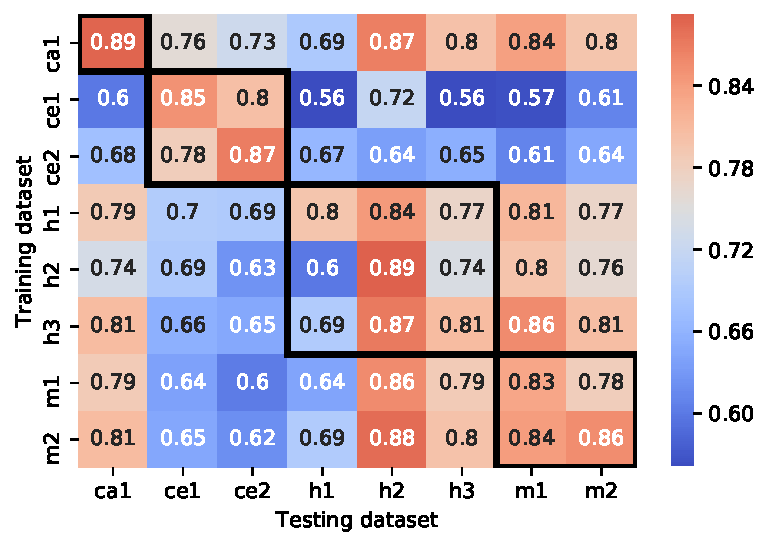
\includegraphics[width = 1\textwidth]{figures/diff_summary_16.pdf}
    \label{fig:crossdataset16}
    \caption*{Each cell \textit{(i,j)} represents the mean accuracy of the 20 classifiers that were trained on 20 training-testing dataset splits of dataset \textit{i} and tested on dataset \textit{j} \textit{ACC(i, j)} using 16 features found in section \textit{Top important features of each dataset}. The black frames surround the results of dataset pairs originating from the same organism.}
      \end{figure}




\begin{table}[h!]
\caption{Intra-dataset classification accuracy with 16 features only}
\label{tab:self_summary16}
\centering
                    \resizebox{\textwidth}{!}{%

\begin{tabular}{|l|l|l|l|l|l|l|}
\hline
Dataset & XGBoost & RF & KNN & SGD & SVM & LR \\ \hline
ca1 & 0.889 (0.004) & 0.889 (0.003) & 0.835 (0.003)        & 0.759 (0.013) & 0.842 (0.003) & 0.771 (0.005) \\ \hline
ce1 & 0.851 (0.015) & 0.85 (0.014)  & 0.782 (0.015)        & 0.778 (0.019) & 0.829 (0.015) & 0.794 (0.017) \\ \hline
ce2 & 0.87 (0.017)  & 0.868 (0.017) & 0.809 (0.014)        & 0.817 (0.032) & 0.859 (0.016) & 0.837 (0.015) \\ \hline
h1  & 0.796 (0.007) & 0.792 (0.006) & 0.748 (0.008)        & 0.733 (0.011) & 0.784 (0.008) & 0.743 (0.008) \\ \hline
h2  & 0.892 (0.012) & 0.885 (0.008) & 0.852 (0.009)        & 0.861 (0.021) & 0.884 (0.009) & 0.881 (0.008) \\ \hline
h3  & 0.809 (0.009) & 0.805 (0.007) & 0.761 (0.011)        & 0.711 (0.047) & 0.804 (0.004) & 0.754 (0.007) \\ \hline
m1  & 0.832 (0.013) & 0.833 (0.015) & 0.746 (0.018)        & 0.71 (0.071)  & 0.808 (0.014) & 0.762 (0.016) \\ \hline
m2  & 0.855 (0.004) & 0.848 (0.004) & 0.808 (0.003)        & 0.785 (0.015) & 0.845 (0.004) & 0.794 (0.004) \\ \hline
\end{tabular}}
\bigbreak
\caption*{Intra-dataset classification accuracy performed with different machine learning methods that incorporate only 16 features identified in section \textit{Top important features of each dataset}. 
The cells contain the mean and the standard deviation (in brackets) values of the accuracy results acquired from 20 models that were trained and evaluated on different training-testing dataset splits.}
\end{table}

